\documentclass[a4paper,12pt,notitlepage]{article}
\usepackage{mathtools}
\usepackage{amssymb}
\usepackage{braket}
\usepackage{graphicx}
\usepackage[section]{placeins}
\title{Data Analysis}
\author{Richard Fox}
\date{}

\begin{document}

\maketitle

\section{Spotting Fake Data}

\begin{figure}[h]
\centering
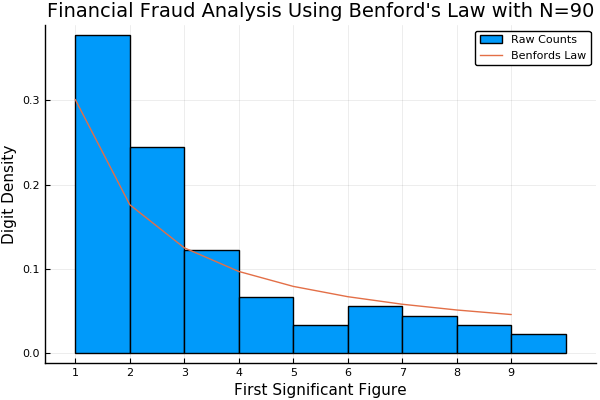
\includegraphics[width=\textwidth]{Benford_90.png}
\caption{Each bar represents the raw count of the first digit equal to the digit on the lower left corner, as is true for the line of Benford's law}
\end{figure}

With sample size of 90, we can see that it fails to reject the null hypothesis (of being from then same kind of distribution) for Benford's law. When increasing to a sample of 900 both the uniform and Benford's law are rejected. At first trying to blindly use the equation provided in the notes led to all results being rejected, even out of range of Julia's default 64 bit precision, i.e. simply yielding $p=0$, as seen in Figure 3. 

\begin{figure}[h!]
\centering
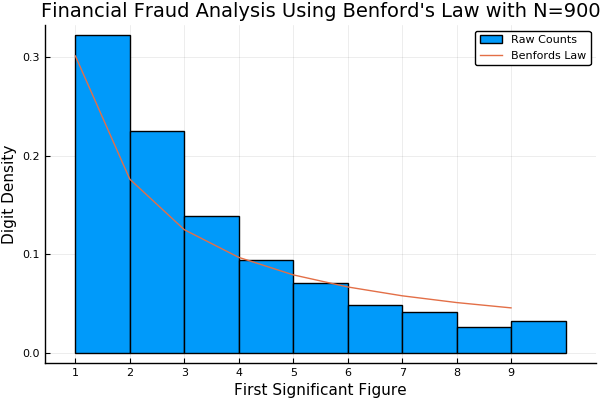
\includegraphics[width=\textwidth]{Benford_900.png}
\caption{Same as Figure 1, but with a sample of 900}
\end{figure}

This is due to the code actually using distributions (fractional counts) as opposed to observations (raw counts), which was discovered by using an package built $\chi ^2$ test which returned an object called "Pearson's Chi Square Test". Upon further research it was realised that a fractions representation of the raw counts needed to be used in the equation, as well as a multiplicative N correction. Now the implemented equations match to package built test (to the first couple of significant figures at least), as well as having an extractable, and therefore useful, P-value, and the reason for the test not working for this higher N became apparent. 

Which is to say that instead of a balancing of over estimation for the low digits and under for the higher ones, the distances from the true null hypothesis distribution are relatively larger therefore falling out of the evaluation 95\% confidence interval once again. 

\begin{figure}[h]
\centering
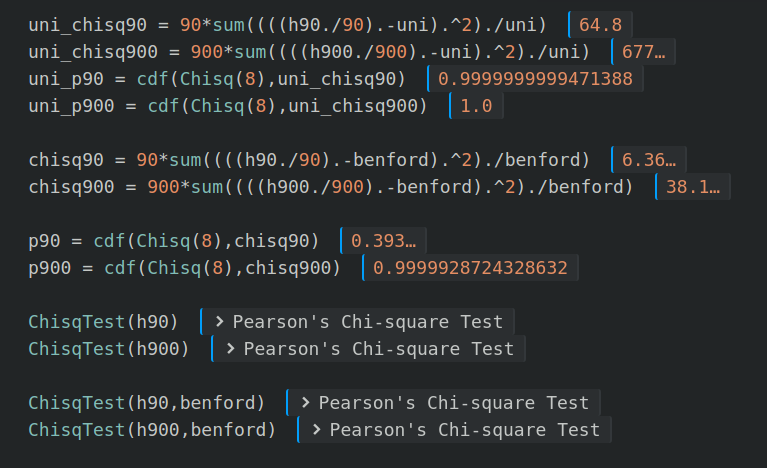
\includegraphics[width=\textwidth]{chisq_code.png}
\caption{Julia code that implements a Pearson $\chi^2$ test by first evaluating the test statistic and then extracting the P-value from the cumulative distribution function, N.B. the $uni\_p900$ value is believed to have fallen out of range for a 64 bit floating point number}
\end{figure}

\section{One and Two Sided Tests}


As we are interested in whether the school is under-performing, for the one sided test the lowest 1\% and 5\% are taken, although the Z-test naturally constructs a distribution that is centred on $0$, so there is only a sign difference from the highest 1\% and 5\%, as we can see with the two-sided values (Figure4).
\begin{figure}[h]
\centering
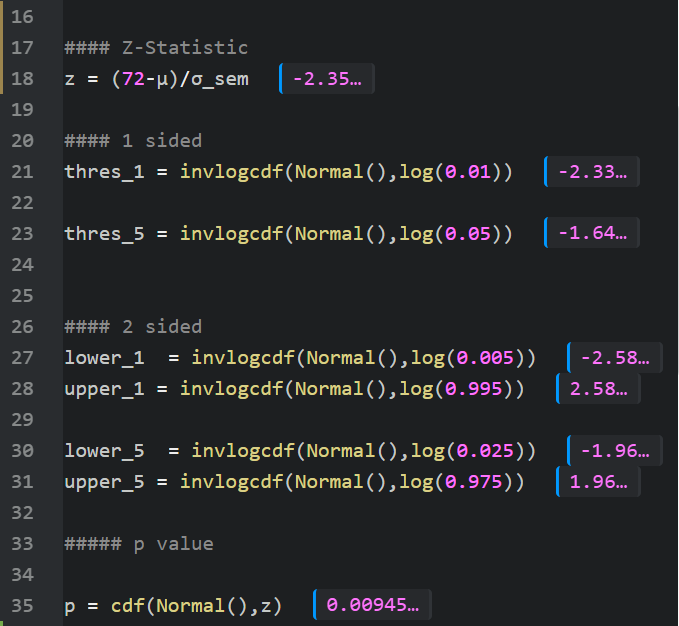
\includegraphics[width=\textwidth]{Z-tests.png}
\caption{The values for a one-sided (thres) and  two-sided (upper, lower) significance tests at both $95\%$ (\_5) and $99\%$ (\_1) for a normal distribution with $\mu = 75$ and $\sigma^2 = 7$, also shown are the Z statistic ($z$) and its P-value ($p$).}
\end{figure}

With this information set out it is fairly straightforward to draw our conclusions, with a one-sided test the school is under-performing with a significance of both 1\% and 5\%, and with the two sided test the school is under-performing with a significance of 5\%, but not to a significance of 1\%.

The P-value confirms this as is less than $0.01$ but greater than $0.005$.

\section{Student's T Test}

$$f(t) = \frac{1}{\sqrt{\nu\pi}} \frac{\Gamma{\big(\frac{\nu - 1}{2}}\big)}{\Gamma{\big(\frac{\nu}{2}}\big)} \frac{1}{(1-\frac{t^2}{\nu})^{\frac{\nu-1}{2}}}$$

Using Sterling's approximation:

$$\frac{\Gamma{\big(\frac{\nu - 1}{2}}\big)}{\Gamma{\big(\frac{\nu}{2}}\big)} = \frac{\sqrt{\frac{2\pi}{\frac{\nu}{2}+\frac{1}{2}}}}{\sqrt{\frac{2\pi}{\frac{\nu}{2}}}}  
 \frac{\bigg(\frac{\frac{\nu}{2}+\frac{1}{2}}{e}\bigg)^{\frac{\nu}{2}+\frac{1}{2}}}{\bigg(\frac{\frac{\nu}{2}}{e}\bigg)^{\frac{\nu}{2}}}$$

$$=\bigg(\frac{\nu+1}{\nu}\bigg)^{\frac{\nu}{2}} \bigg(\frac{\nu}{2}\bigg)^{\frac{1}{2}} e^{-\frac{1}{2}} = \bigg(1+\frac{\frac{1}{2}}{\frac{\nu}{2}}\bigg)^{\frac{\nu}{2}} \bigg(\frac{\nu}{2}\bigg)^{\frac{1}{2}} e^{-\frac{1}{2}} = \bigg(\frac{\nu}{2}\bigg)^{\frac{1}{2}}$$

Subbing this back into $f(t)$ and looking for the form of an exponential again (to match the normal distribution) yields:

$$f(t) = \bigg(\frac{\nu}{\nu}\bigg)^{\frac{1}{2}} \frac{1}{\sqrt{2\pi}} \bigg(1-\frac{t^2}{\nu}\bigg)^{-\frac{\nu-1}{2}}$$

$$ = \frac{1}{\sqrt{2\pi}} \bigg(1-\frac{t^2}{\nu}\bigg)^{\frac{1}{2}} \bigg(1-\frac{\frac{t^2}{2}}{\frac{\nu}{2}}\bigg)^{-\frac{\nu}{2}}$$ 

$$ = \frac{1}{\sqrt{2\pi}} \bigg(1-\frac{t^2}{\nu}\bigg)^{\frac{1}{2}} e^{-\frac{t^2}{2}}$$

As we are taking the limit as $n \rightarrow \infty$ in which case $ \nu \rightarrow \infty$ meaning the term $\bigg(1-\frac{t^2}{\nu}\bigg)^{\frac{1}{2}} \rightarrow 1$ leaving us with a normal distribution:

$$ \lim_{n \to \infty} f(t) = \frac{1}{\sqrt{2\pi}} e^{-\frac{t^2}{2}}$$

The variance of the Student's t distribution is defined as $\sigma^2 := \frac{\nu}{\nu-2}$ and utilising a Laurent expansion yeilds:

$$ \frac{\nu}{\nu-2} = 1+ \frac{2}{\nu}+ O\bigg(\frac{1}{\nu^2}\bigg)$$

Which will tend to the normal distribution variance of 1 but from a higher value giving it a greater error when not in the limit of $n \to \infty$

\section{Maximum Likelihood (Normal Dist.)}

The likelihood of sample data parameters describing the population parameters is written as :

$$ \mathbb{P}[\Vec{X}\ |  \mu ,\sigma   ], $$

where $\mu$ and $\sigma$ are the true population mean and standard deviation respectively, and $\Vec{X} = [X_1 \dots X_n]$ is the sample data. Using the probability distribution function (PDF) for a Normal Distribution we show the likelihood is given by:

$$\mathbb{P}[\Vec{X}\ |  \mu ,\sigma   ] = \frac{1}{\sqrt{2\pi\sigma^2}}\exp{-\frac{(\Vec{X}-\mu)^2}{2\sigma^2}}$$

Taking the logarithm (giving the log-likelihood) allows use to do several transformations to our equation:

$$=\ln\bigg(\frac{1}{\sqrt{2\pi\sigma^2}}\exp{-\frac{(\Vec{X}-\mu)^2}{2\sigma^2}}\bigg)$$
$$=-\frac{n}{2}\ln{(2\pi\sigma^2)}-\sum_{i=1}^{n}-\frac{(X_i-\mu)^2}{2\sigma^2}$$
$$=-\frac{n}{2}\ln{(2\pi)}-n\ln{(\sigma)}-\sum_{i=1}^{n}-\frac{(X_i-\mu)^2}{2\sigma^2}$$
Now we hold $\sigma$ constant and take the derivative with respect to $\mu$ and set it $=0$ to find the maximal likelihood for $\hat{\mu}$ :

$$\frac{\partial\mathbb{P}[\Vec{X}\ |  \mu ,\sigma   ]}{\partial\mu}=0-0-\sum_{i=1}^{n}-\frac{(X_i-\hat{\mu})}{\sigma^2} = 0$$
$$ \frac{1}{\sigma^2}[\Vec{X} - n\hat{\mu}] =0$$
$$\hat{\mu} = \frac{1}{n}\sum_{i=1}^{n}X_i$$

Holding $\mu$ as a constant at $\hat{\mu}$ and pulling the same trick for $\sigma$ to find $\hat{\sigma}$ :

$$\frac{\partial\mathbb{P}[\Vec{X}\ |  \mu ,\sigma   ]}{\partial\sigma}=0-\frac{n}{\hat{\sigma}}-\sum_{i=1}^{n}-\frac{(X_i-\hat{\mu})^2}{\hat{\sigma}^3} = 0$$

$$\hat{\sigma}^2 =\frac{1}{n} \sum_{i=1}^{n}(X_i-\hat{\mu})^2 $$


To show bias we need the expectation of the estimator to equal what it is estimating in this case the variance $\sigma^2$, i.e. $\mathbb{E}[\hat{\sigma}^2] = \sigma^2$.

$$\mathbb{E}[\hat{\sigma}^2] = \mathbb{E}\bigg[\frac{1}{n} \sum_{i=1}^{n}(X_i-\hat{\mu})^2\bigg]$$

$$ = \frac{1}{n} \sum_{i=1}^{n}(\mathbb{E}[X_i^2] - 2\mathbb{E}[X_i \hat{\mu}] + \mathbb{E}[\hat{\mu}^2])$$

The definition of variance is $VAR(X) = \mathbb{E}[X^2] - \mathbb{E}[X]^2$ where $VAR(X) = \sigma^2$ and $\mathbb{E}[X]^2 = \mu^2$ leaving :
$$\mathbb{E}[X^2] = \sigma^2 + \mu^2,$$

now for $\mathbb{E}[\hat{\mu}^2]$ can be rewritten as a double sum and then thought of as a matrix with only the diagonal having non-zero entries or $\sigma^2$ :

$$\mathbb{E}[\hat{\mu}^2] = \frac{1}{n^2} \sum_{i=1}^n \sum_{j=1}^n \mathbb{E}[X_i X_j] = \frac{1}{n^2} (n^2 \mu^2 + n \sigma^2) = \mu^2 + \frac{\sigma^2}{n}, $$

using a similar trick and the definition of $\hat{\mu}$ we obtain:

$$ \mathbb{E}[X_i \hat{\mu}] = \frac{1}{n} \sum_{j=1}^n \mathbb{E}[X_i X_j] = \frac{1}{n} (n\mu^2 + \sigma^2) = \mu^2 + \frac{\sigma^2}{n}.$$

Plugging these back into our main equation gives:

$$ \mathbb{E}[\hat{\sigma}^2] = \frac{1}{n} \sum_{i=1}^n \big[ \mu^2 + \sigma^2 - 2(\mu^2 + \frac{\sigma^2}{n}) + \mu^2 + \frac{\sigma^2}{n}\big]$$

$$ = \frac{1}{n} n \big[ \sigma^2 - 2 \frac{\sigma^2}{n} + \frac{\sigma^2}{n}\big] = \big(1-\frac{1}{n}\big)\sigma^2$$

showing that our estimator for the maximum likelihood is indeed a biased estimator.

\section{Bayesian Posterior (Normal Dist.)}

The population mean and variance used here are $\mu=5 , \  \sigma^2=0.25$, and using a 100x100 grid of values, where $\mu \in [1,10] , \ \sigma \in [0.1,1]$. The ranges were chosen to help avoid sign mistakes and make plotting easier, by keeping $\mu$ positive we avoid needing a centre axis, and keeping $\sigma < 1$ keeps both $\sigma$ and $\sigma^2$ over roughly the same range, that is to say that strictly $\sigma^2 \in [0.01,1]$.

\begin{figure}[h]
\centering
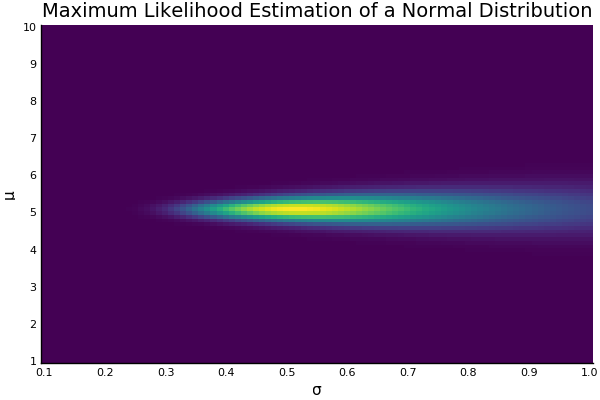
\includegraphics[width=13cm,8cm]{mle_2d.png}
\caption{The x axis here is $\sigma$ and not $\sigma^2$ as it is more convenient to input into the Julia function for normal distributions as they require the standard deviation}
\end{figure}

\begin{figure}[h]
\centering
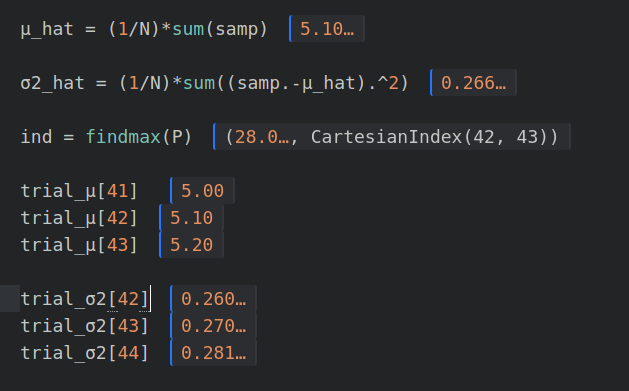
\includegraphics[width=13cm,8cm]{hatvalues.png}
\caption{Maximum likelihood values for the sample, based on section 4, and the corresponding values at the indexes for the highest likelihood value}
\end{figure}

The indexes at which the maximum likelihood occurred appear to be the closest matches for the analytic estimators available (Figure 6). Also the peaks of marginals taken at these points do indeed appear to coincide with the analytic predictions for both parameters (Figure 7 and Figure 8).
\begin{figure}[h]
\centering
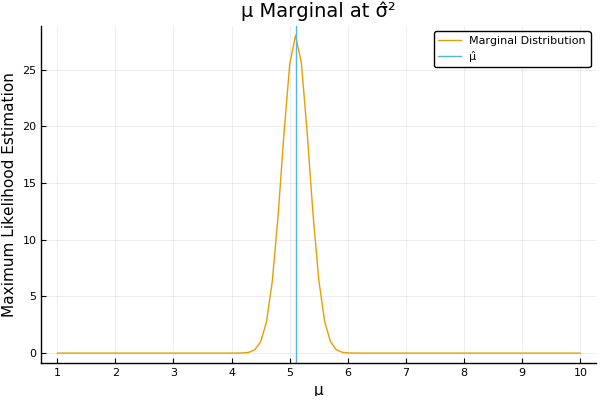
\includegraphics[width=13cm,8cm]{mu_marginal.png}
\caption{The y axis corresponds to the result of the posterior at each value of $\mu$ evaluated, although quite sharp there is evidence of the normally distributed sample means}
\centering
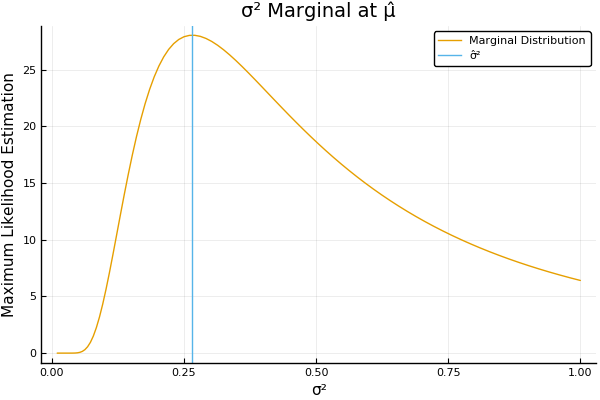
\includegraphics[width=13cm,8cm]{sigma_marginal.png}
\caption{The same as Figure 7 but for $\sigma^2$, but has the distribution we would expect from a squared variable, i.e. fatter right hand tail and strictly above 0}
\end{figure}

\end{document}